\chapter{Electronics}
\label{ch:elec}
The pulse signals produced by the silicon detectors in HELIOS are the characteristic charge-collection pulses produced by semiconductor detectors; a low-amplitude pulse with a fast rise-time and a slow decay.  The data acquisition system requires that the detector pulses be digitized in some way; specifically, the amplitude of the pulse is converted into a number stored by the computer system.  In order to be digitized, the detector pulses must be processed.  Each detector signal passed through a linear amplifier (preamplifier) before a shaping amplifier is used to produce a pulse shape suited to digitizing.  The signal processing performed by the shaping amplifier also produces a timing signal which is used to create a logic trigger.  Both of these processes are described in this chapter.  The use of position-sensitive detectors in HELIOS---as opposed to segmented detectors---reduces the number of electronics channels that are read out from the array.  The reduced amount of hardware required allows for a streamlined electronics setup described below.  
%Each of the 24 detectors which comprise the HELIOS detector array has three signals which are read out The entire prototype array can be read out with nine 8-channel preamplifiers.  

\section{Patch Boards}
Each of the four PC boards which make up the array is connected to an electronics feedthrough by two 94.1\,cm-long ribbon cables (see Fig.~\ref{array_pic}).  This is the shortest length of cable that allows a full range of motion for the array.  The cables are terminated by 34-pin micro IDC header sockets.  This configuration was used with the prototype array to accommodate, and thus provide compatibility with, 30 signals per board.  The electronics feedthroughs, shown in Fig.~\ref{feedthrough}, pass through a slot in a modified feedthrough cap and are held in place with sealing epoxy.

On the atmosphere side of the feedthrough, stock aluminum card guides are used for mechanical support.  The electronics feedthrough serves as a patch board to distribute the detector signals.  Each board has three rows of 10 LEMO sockets, with each row corresponding to a detector signal: $E$, $X_\textrm{far}$, and $X_\textrm{far}$.  The energy-signal connectors are mounted on the back side of the patch board so that the LEMO plugs can be inserted and removed by hand (without using tools).  An additional two LEMO connectors are present to read and power the temperature sensor at the target-end of each array PC board.  
\begin{figure}[t]
\centering
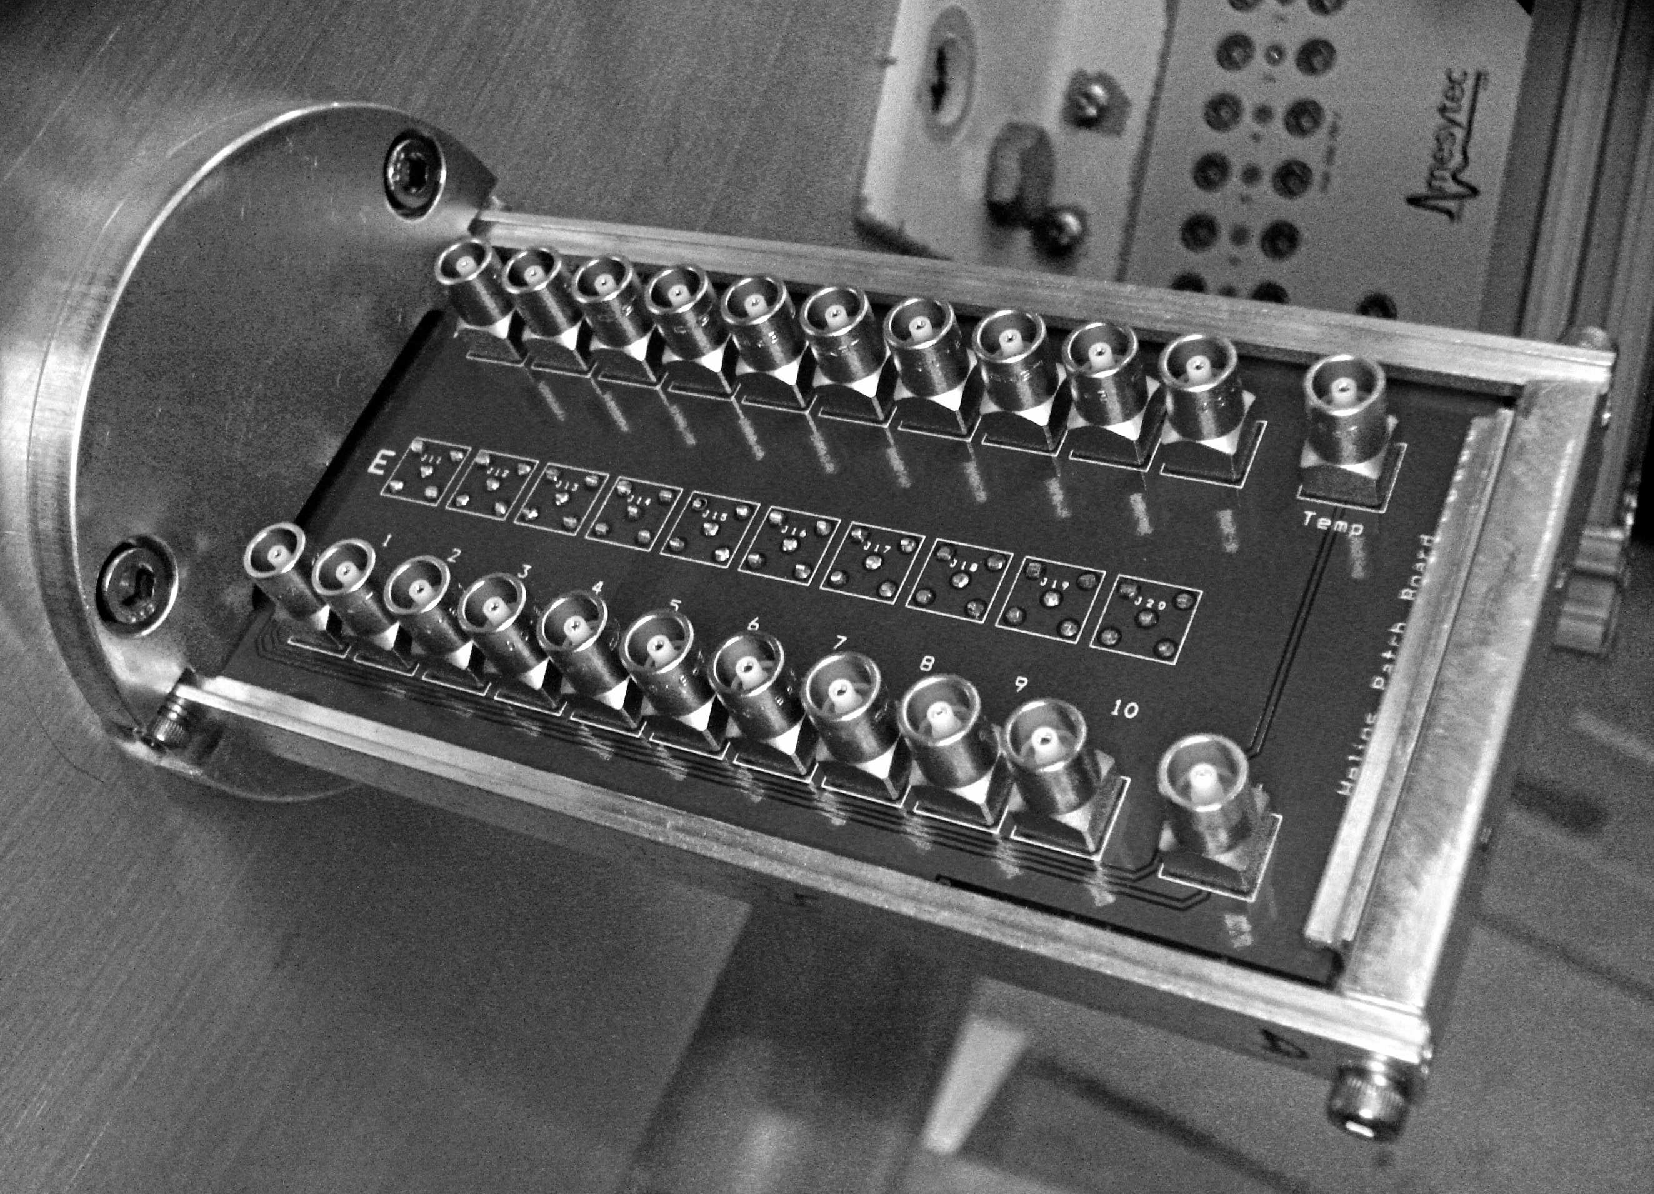
\includegraphics[height=0.33\textheight,width=0.48\linewidth,keepaspectratio]{DSC01506}~
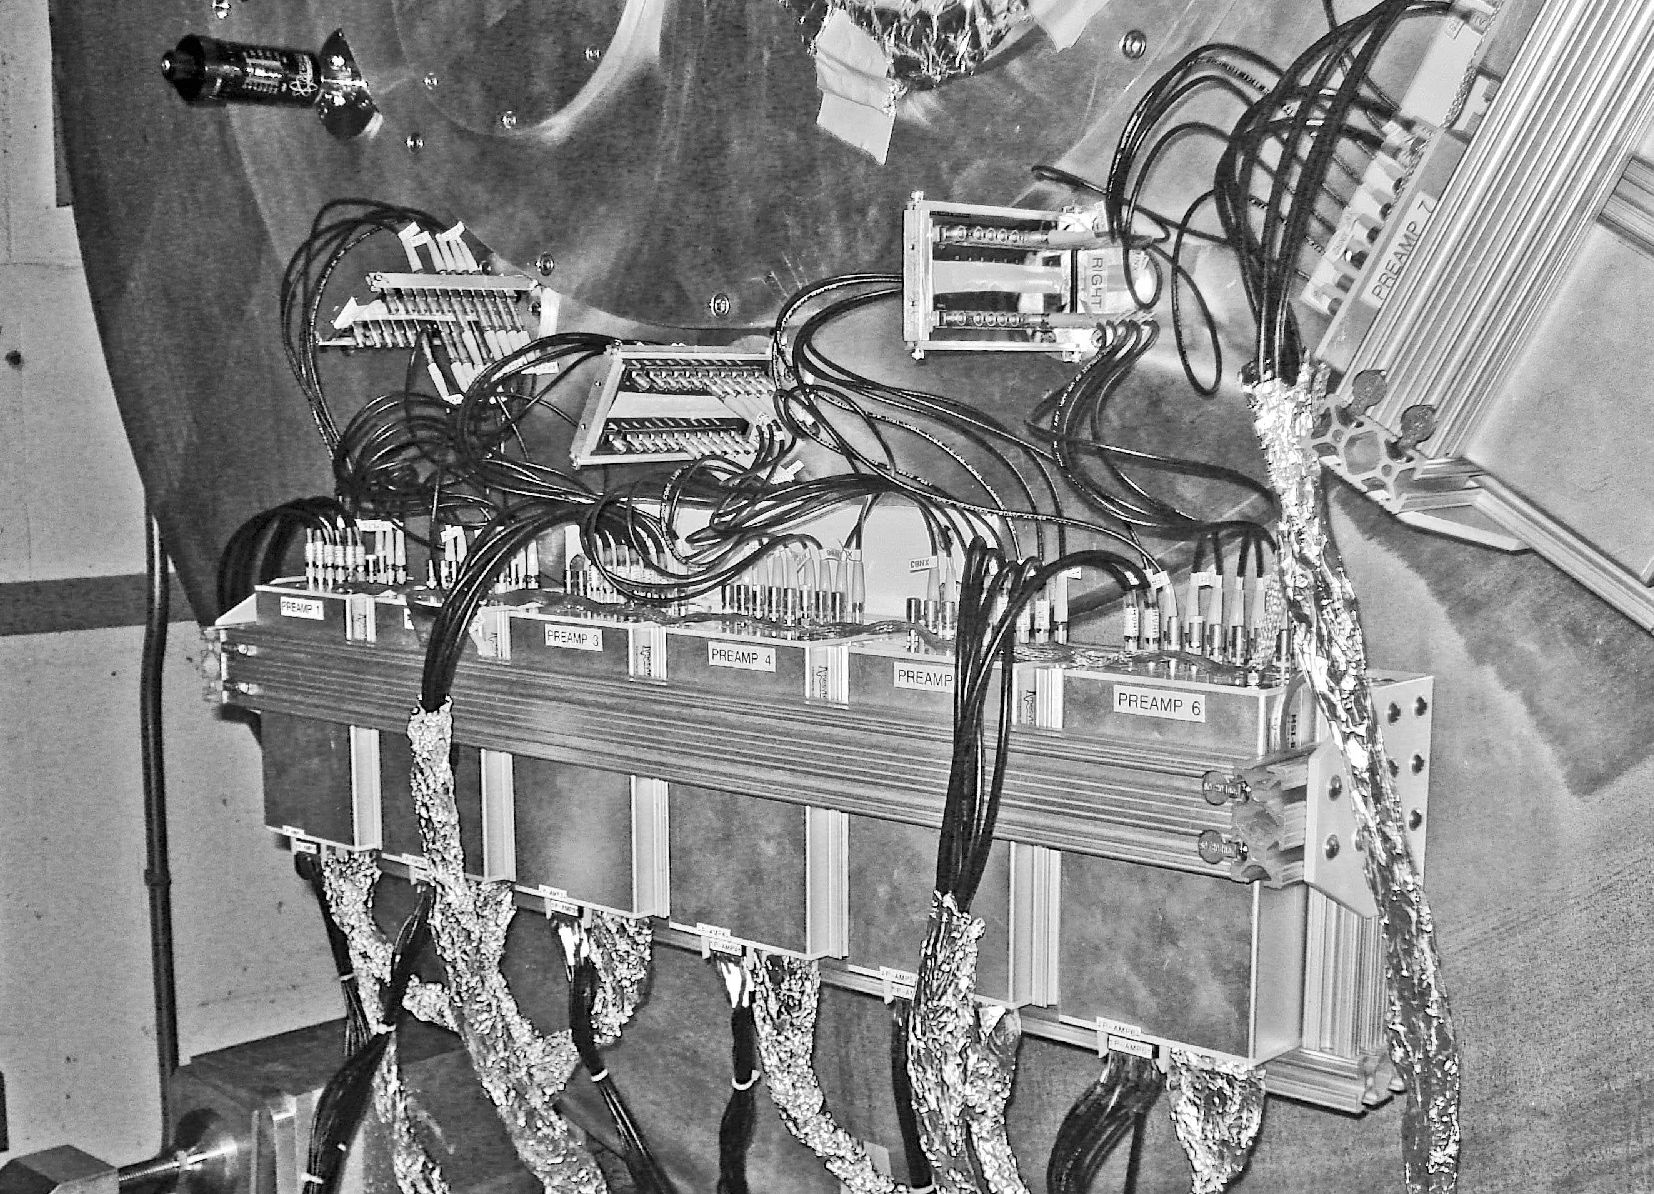
\includegraphics[height=0.33\textheight,width=0.48\linewidth,keepaspectratio]{DSC01945_bw}
\caption[The HELIOS detector array electronics feedthroughs]{The HELIOS detector array electronics feedthroughs.  (left) Each patch board features 32 LEMO connections.  (right) Three of the four patch boards connected to their respective preamplifiers by 54 40\,cm-long LEMO cables.}%
\label{feedthrough}%
\end{figure}
\section{Signal Processing}
\subsection{Preamplifiers}
The detector array signals from the feedthrough patch boards are first processed with a Mesytec MSI-8p preamplifier.  Each preamplifier has eight input channels and each PC board has 18 output channels, so each patch board is connected to three preamplifiers, nine in total. Fig.~\ref{feedthrough} shows a photograph of the preamplifier as they are installed and Fig.~\ref{emap} is a connection diagram.  The preamplifiers are mounted to the front flange of the solenoid to bring them as close as possible to the feedthrough patch boards.  The supports for the preamplifiers are largely made out of material re\-pur\-posed from the field mapping jig.  The connection between patch boards and preamplifiers is made with 40\,cm coaxial cables constructed with specialized low-loss transmission RG-174 cables\footnote{Belden 7805 25\,AWG solid-core coaxial wire with tinned copper braided shielding and aluminum foil-polyester tape shielding.} and terminated with LEMO connectors.  Such care is taken with shielding the cables and minimizing the cable length in order to preserve shape of the un-amplified signals from the detectors.

\begin{figure}[t]
\centering
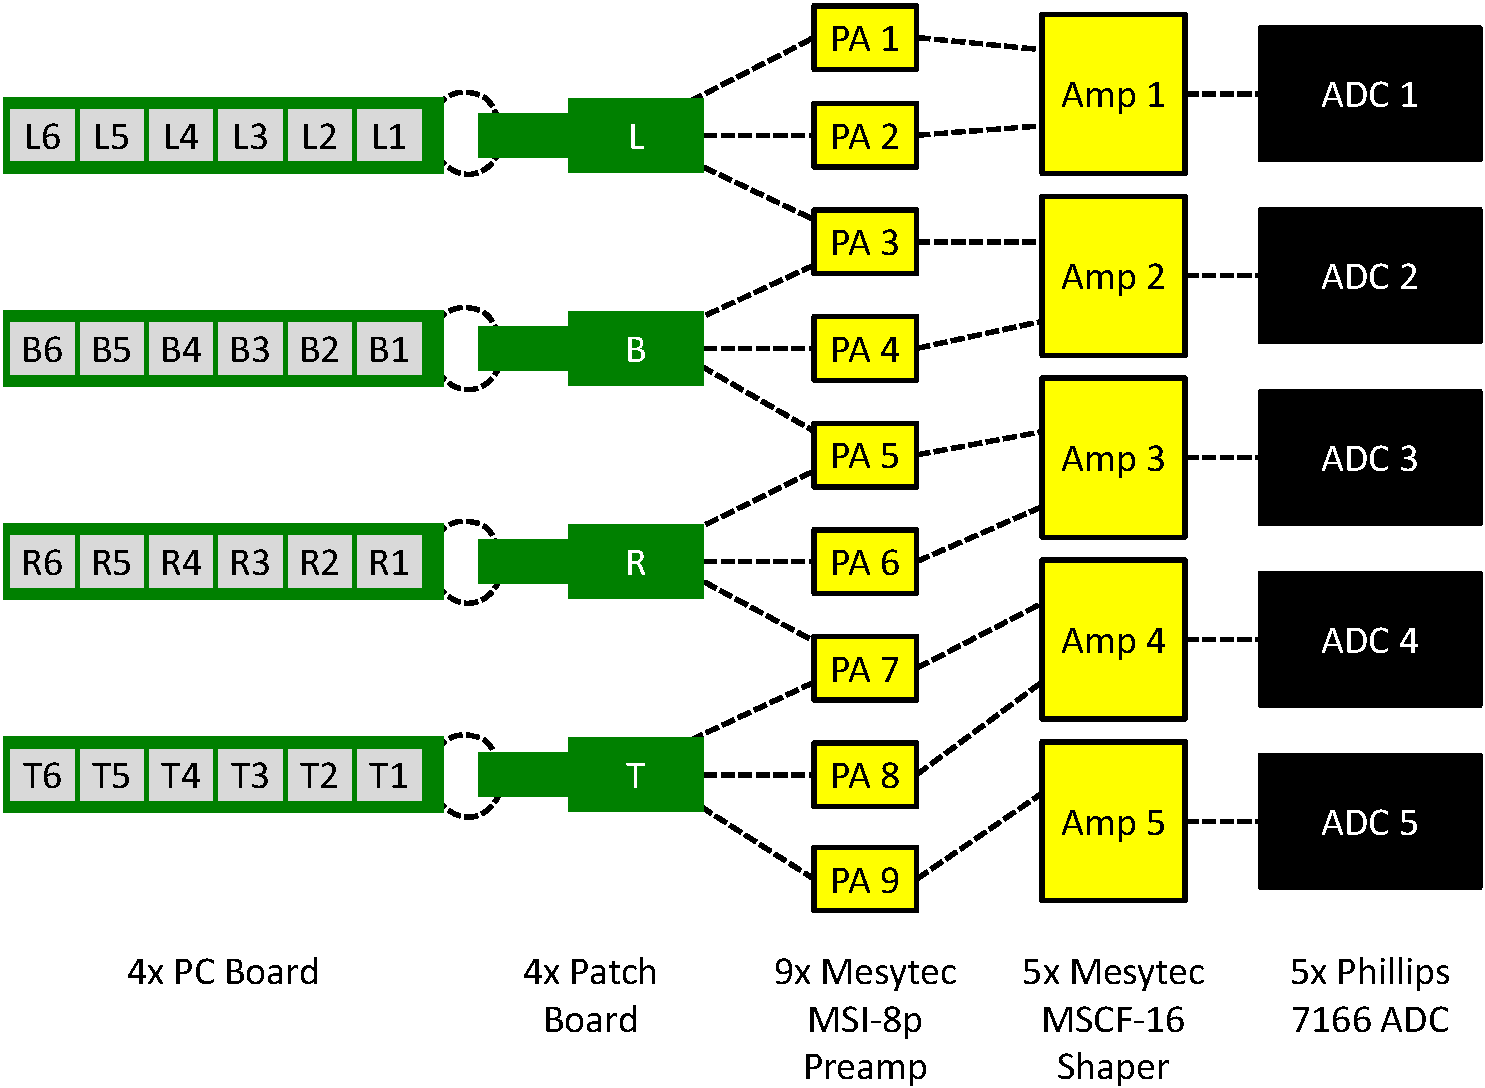
\includegraphics[width=\columnwidth]{emap}%
\caption[Schematic diagram of the electronics for signal processing]{Schematic diagram of the electronics for signal processing.  Detectors are numbered 1--6 on each side of the array, starting at the feedthrough-end of the array.  Each detector array PC board connects to a dedicated feedthrough patch board.  The patch boards each connect the to three preamplifiers which are in turn connected to the shaper amplifiers in pairs.  Each amplifier has a dedicated ADC.  }%
\label{emap}%
\end{figure}

The detectors are reverse-biased through the energy contact with the position contacts terminated into 50\,$\Omega$.  For the commissioning experiment, the detectors were biased using a collection of Ortec Model 210 Detector Control Unit 4-channel high voltage bias supplies.  Subsequent experiments utilized an Iseg High Voltage Mpod-mini computer controlled multi-channel bias supply.  Both the bias supply and the power supply for the preamplifiers are positioned in a region of lower magnetic field at a distance of about 1.5\,m from the flange face of the solenoid.  As a result of this significant separation, specialized shielded DB9 connectors had to be used to power the MSI-8p preamplifiers.

\subsection{Shaping Amplifiers}
The 8-channel preamplifiers are connected in pairs to 16-channel Mesytec MSCF-16 shaper amplifiers, five in all.  The shaping amplifier is of type $CR-(RC)^5$, meaning a single stage of $CR$ differentiation followed by 5 stages of $RC$ integration to produce a nearly Gaussian output waveform.  The amplifiers provide gain and shaping time adjustment in 4-channel blocks, while threshold and pole-zero cancellation adjustments are made for each channel. Pole-zero cancellation is an automatic process while setting the threshold of each channel is done manually.  Thresholds are set to minimize or eliminate trigger on baseline noise.

In terms of bulk signal processing, the amplifier modules have one input and two outputs, each consisting of a 34-pin header.  The incoming and outgoing energy signals are carried on shielded cables (RG-174) to reduce signal noise and because the shape of the signals is important.  The shaper output is connected to a peak-sensing analog-to-digital converter (ADC). The timing signal, which is a logic pulse, is output over a standard 34-conductor, braided-pair ribbon cable.  The timing signals are used to generate an event trigger.%  Fig.~\ref{emap} is a connection diagram for the electronics readout.

\section{Triggering}
The Mesytec MSCF-16 shaper amplifiers contain timing filter amplifier (TFA) and constant fraction discriminator (CFD) circuitry to produce timing signals.  When the discriminator threshold of an individual detector is exceeded, a timing  signal, or trigger, is produced.  The output signals are of the form of emitter-coupled logic (ECL) signals.  The 16-channel ECL timing output from each shaping amplifier module is connected to a level translator.  The level translators---typically a LeCroy 4616 or a Phillips 726---are used to convert the ECL input signal to a nuclear instrumentation module (NIM) output signal.  Fig.~\ref{emap2} shows a typical connection diagram used for producing the event trigger.

\begin{figure}
\centering
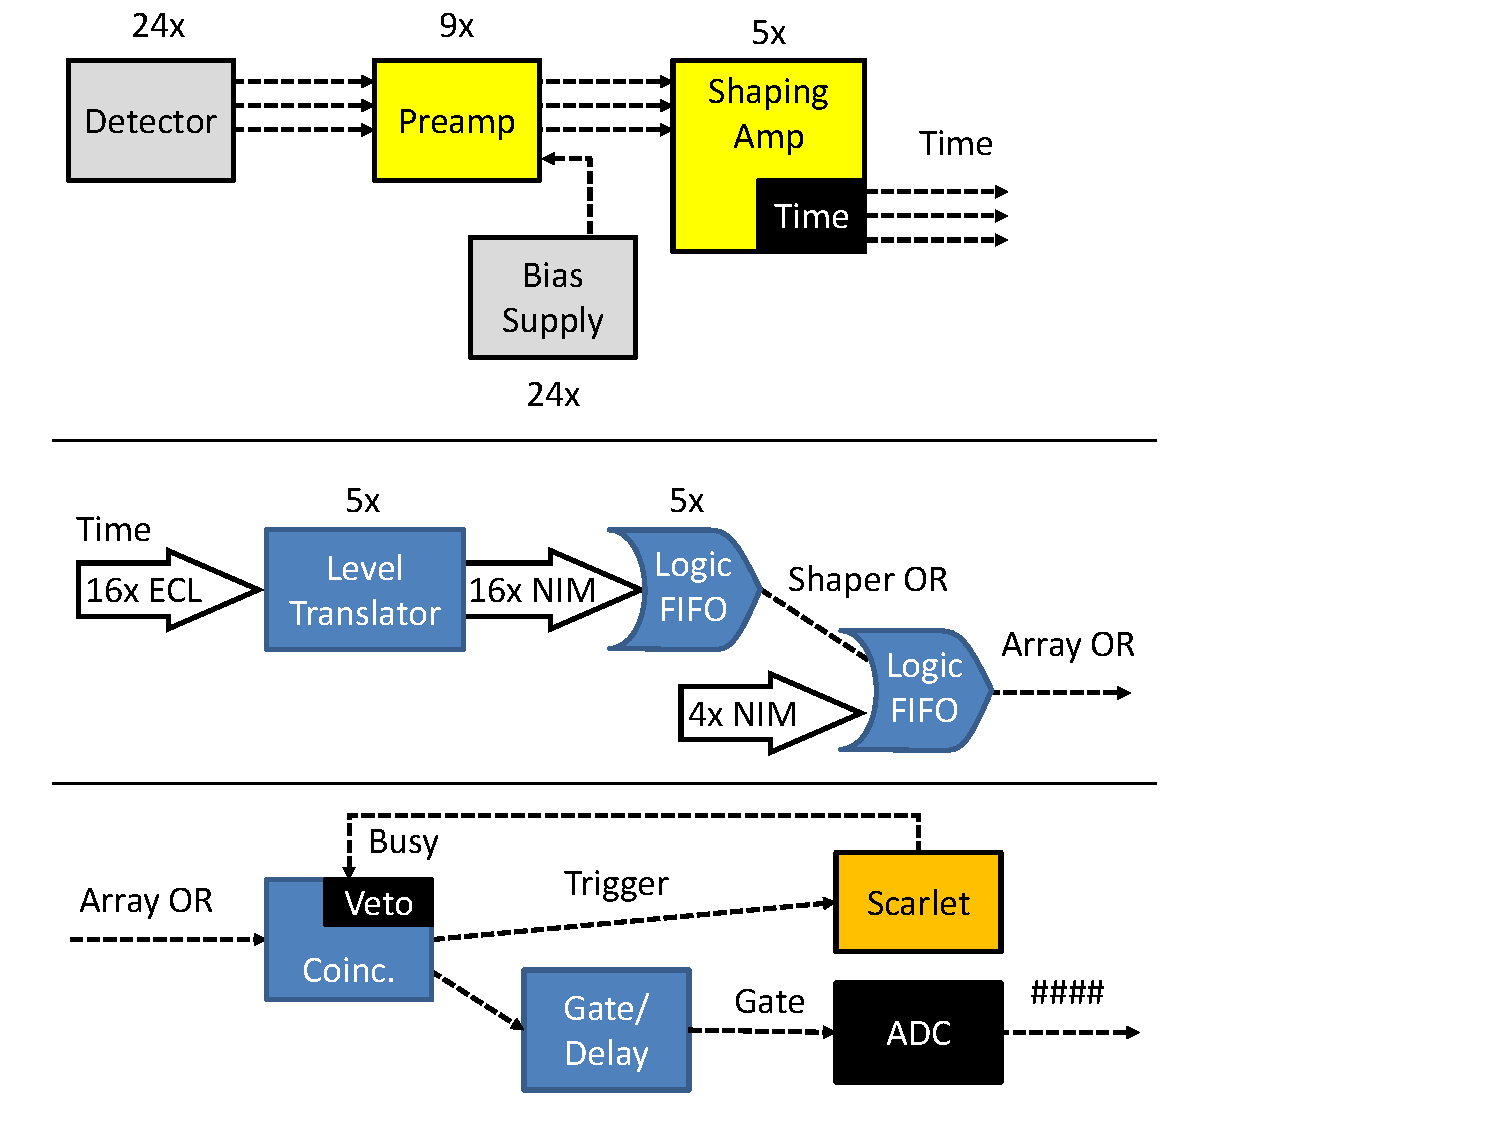
\includegraphics[width=\columnwidth,height=0.5\textheight,keepaspectratio]{electronics_diagram2}%
\caption[Schematic diagram of the electronics producing the event trigger]{Schematic diagram of the electronics  producing the event trigger.  Each detector has three signals which are preamplified before being processed by a shaping amplifier.  The shaping amplifier includes a CFD to produce timing signals for each detector.  The ECL timing signals are converted to NIM signals and are ORed together by a logic fan-in/fan-out (FIFO) module.}%
\label{emap2}%
\end{figure}

The level translators are used as a switchboard to select which signals are included in the event trigger.  The individual outputs from each level translator (up to 16 signals) are fed into a logic fan-in/fan-out module, which acts to produce the logical `OR' of the timing pulses from each shaping amplifier module. The outputs from each of the five logic fan-in/fan-out modules are ORed together again to produce "Array OR" trigger signal.

The time of flight measurement is generated based on the Array OR trigger.  The master RF signal used to drive the accelerator resonators (a sine wave) is put through a level discriminator to generate narrow, square pulses with a period equal to 82\,ns.  This RF timing signal serves as the \textit{start} signal on a time-to-amplitude converter (TAC).  A delayed version of the Array OR signal is then used as the \textit{stop} signal for the TAC.

In the commissioning experiment, only the energy signals---and only those with low noise---were used to establish an event trigger.  For measurements involving additional detectors, for instance a recoil detector, the trigger signals from those additional detectors would also enter into the event trigger; either in two-fold coincidence with the array trigger or in fan-out (``singles'') mode.  
Once the event trigger is generated, it is used to start the Scarlet data acquisition system, discussed below.  During the acquisition process, the Scarlet system issues an ``busy'' signal to inhibit the generation of new triggers while acquisition is taking place.  For this reason, the event trigger is generated using a coincidence module which requires the absence of an inhibit signal to produces coincidences.

\section{Acquisition}
\label{acq}
The energy signals from the Mesytec shaper amplifiers modules are each connected to a dedicated Phillips 7166H (``H'' for ``header'') peak-sensing ADC.  The event trigger is used to start the acquisition, gate the ADCs, and is also counted in a scaler to monitor the event rate.  Using a gate and delay generator, the event trigger is delayed and broadened to produce a logic signal which overlaps in time with the shaped pulses from the Mesytec shaper amplifiers.  The amplitude of the pulse within the gate is converted by the ADC into a 12-bit number.

For each event trigger, the Scarlet acquisition system issues a series of readout commands to a Weiner CC32 CAMAC controller which communicates with the individual CAMAC modules, such as the ADCs.  Each ADC corresponding the detector array is interrogated for the number of channels with successful conversions, or ``hits.'' Only those channels with hits are read out. Additional ADCs, which may be used to read out signals  are read out sequentially with each channel being read.  As this process occurs, the Scarlet system inhibits further events triggers until the current event has been processed.  Once complete, the busy signal is cleared and acquisition continues.